The power supply layer is one if not the most important layer because it provides stable power supply to the cart. The parts in this subsystem are responsible for powering every other subsystem and any external tools or equiment. 

\begin{figure}[h!]
	\centering
 	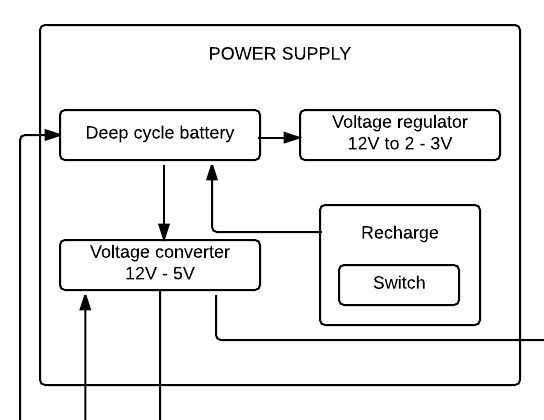
\includegraphics[width=0.60\textwidth]{images/power_supply}
 \caption{Power supply layer}
\end{figure}

\subsection{Deep Cycle Battery}
The deep cycle battery is designed to power everything. Once the cart's switch is turned on, the deep cycle battery will then begin to power the other subsystems on.

\begin{figure}[h!]
	\centering
 	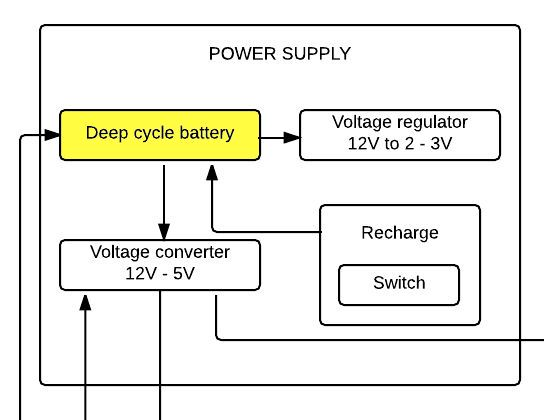
\includegraphics[width=0.60\textwidth]{images/power_supply_batt}
 \caption{Deep cycle battery subsystem}
\end{figure}

\subsubsection{Assumptions}
Assumptions made are as follows:
\begin{itemize}
	\item The battery is charged.
	\item The battery is properly connected to the cart.
	\item The battery is fully functional.
	\item The battery is connected to the cart at all times.
	\item The battery will be 12V.
\end{itemize}

\subsubsection{Responsibilities}
The deep cycle battery subsystem's responsibilities are as follows:
\begin{itemize}
	\item Enable stable power to the other subsystems after being converted from 12V to 5V through the voltage converter.
	\item Enable stable power to external tools and equipment after being converted from 12V to 2 - 3V through the voltage regulator.
\end{itemize}

\subsubsection{Subsystem Interfaces}

\begin {table}[H]
\caption {Deep cycle battery subsystem interfaces} 
\begin{center}
    \begin{tabular}{ | p{1cm} | p{6cm} | p{3cm} | p{3cm} |}
    \hline
    ID & Description & Inputs & Outputs \\ \hline
    \ N/A & Power integrated power supply & \pbox{3cm}{N/A} & \pbox{3cm}{Voltage regulator }  \\ \hline
    \ N/A & Power electronic components & \pbox{3cm}{N/A} & \pbox{3cm}{Voltage converter}  \\ \hline
    \ N/A & Safety killswitch & \pbox{3cm}{Killswitch} & \pbox{3cm}{N/A}  \\ \hline
    \ N/A & Safety manual mode & \pbox{3cm}{Manual-mode switch} & \pbox{3cm}{N/A}  \\ \hline
    \end{tabular}
\end{center}
\end{table}

\subsection{Voltage Regulator}
The voltage regulator is designed to convert the 12V voltage from the deep cycle battery to 2 - 3V and it will mainly be used to power up external tools and equipment.

\begin{figure}[h!]
	\centering
 	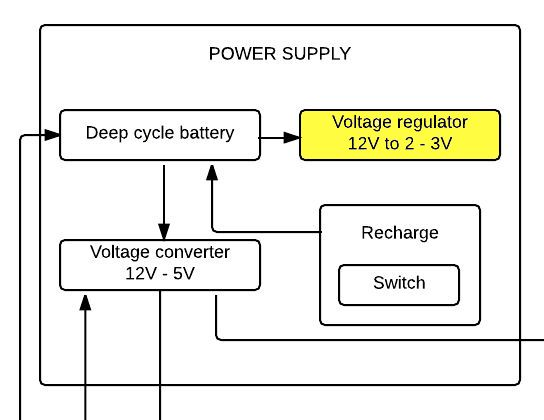
\includegraphics[width=0.60\textwidth]{images/power_supply_regulator}
 \caption{Voltage regulator subsystem}
\end{figure}

\subsubsection{Assumptions}
Assumptions made are as follows:
\begin{itemize}
	\item The voltage from the battery will be 12V.
	\item The voltage required for external tools and equipment will be between 2 - 3V.
\end{itemize}

\subsubsection{Responsibilities}
The voltage regulator subsystem's responsibilities are as follows:
\begin{itemize}
	\item To enable and regulate constant voltage level for powering external tools and supplies.
\end{itemize}

\subsubsection{Subsystem Interfaces}
\begin {table}[H]
\caption {Voltage regulator subsystem interfaces} 
\begin{center}
    \begin{tabular}{ | p{1cm} | p{6cm} | p{3cm} | p{3cm} |}
    \hline
    ID & Description & Inputs & Outputs \\ \hline
    \ N/A & Receive power & \pbox{3cm}{Deep cycle battery} & \pbox{3cm}{N/A}  \\ \hline
    \end{tabular}
\end{center}
\end{table}
\newline

\subsection{Voltage Converter}
The voltage regulator is designed to convert the 12V voltage from the deep cycle battery to 2 - 3V and it will mainly be used to power up the Smart Cart's components.

\begin{figure}[h!]
	\centering
 	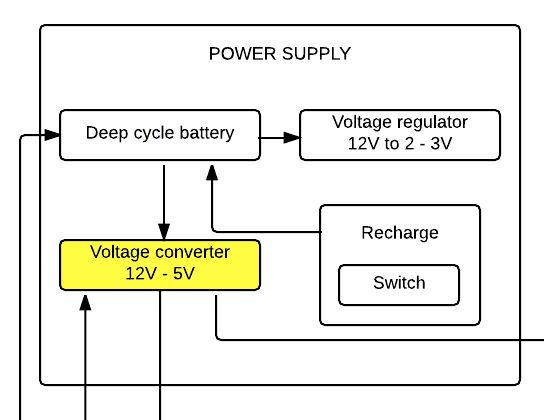
\includegraphics[width=0.60\textwidth]{images/power_supply_converter}
 \caption{Voltage converter subsystem}
\end{figure}

\subsubsection{Assumptions}
Assumptions made are as follows:
\begin{itemize}
	\item The voltage from the battery will be 12V.
	\item The voltage required for the cart's components will be 5V.
\end{itemize}

\subsubsection{Responsibilities}
The voltage converter subsystem's responsibilities are as follows:
\begin{itemize}
	\item Enable stable power to the other subsystems, which include the crab drive system and image processing after being converted from 12V to 5V through the voltage converter.
\end{itemize}

\subsubsection{Subsystem Interfaces}
\begin {table}[H]
\caption {Voltage converter subsystem interfaces} 
\begin{center}
    \begin{tabular}{ | p{1cm} | p{6cm} | p{3cm} | p{3cm} |}
    \hline
    ID & Description & Inputs & Outputs \\ \hline
    \ N/A & Receive power & \pbox{3cm}{Deep cycle battery} & \pbox{3cm}{N/A}  \\ \hline
    \ N/A & Safety manual mode & \pbox{3cm}{Manual-mode switch} & \pbox{3cm}{Crab-drive system \\ Imaging and navigation}  \\ \hline
    \end{tabular}
\end{center}
\end{table}
\newline

\subsection{Recharge}
The recharge subsystem will be used to ensure that the Smart Cart will be charged without having too much electricity going to the electronics or the other battery and cause problems.

\begin{figure}[h!]
	\centering
 	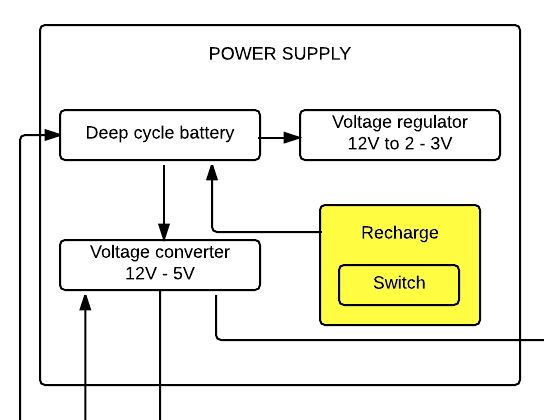
\includegraphics[width=0.60\textwidth]{images/power_supply_recharge}
 \caption{Recharge subsystem}
\end{figure}

\subsubsection{Assumptions}
Assumptions made are as follows:
\begin{itemize}
	\item The recharge subsystem will ensure the safety of the tools and equipment.
\end{itemize}

\subsubsection{Responsibilities}
The recharge subsystem's responsibilities are as follows:
\begin{itemize}
	\item A switch will disable the battery from powering the Smart Cart components while it is being recharged.
\end{itemize}

\subsubsection{Subsystem Interfaces}
\begin {table}[H]
\caption {Recharge subsystem interfaces} 
\begin{center}
    \begin{tabular}{ | p{1cm} | p{6cm} | p{3cm} | p{3cm} |}
    \hline
    ID & Description & Inputs & Outputs \\ \hline
    \ N/A & Switch on safety & \pbox{3cm}{Switch} & \pbox{3cm}{Deep cycle battery}  \\ \hline
    \end{tabular}
\end{center}
\end{table}